\section{Results}
\label{sec:results}

% Table 1: Hypothesis Status
% Source: paper_assets/final_metrics.json + docs/paper_claims.md
\begin{table}[h]
\caption{%
  \textbf{Final hypothesis verdicts (Runs~001--013).}
  H1'' and H3'' are the refined real-data hypotheses replacing the original
  synthetic-KG formulations.
  H2 was validated on synthetic KGs only and not retested on real data.
  H4 required rubric revision (Run~010) before passing.
  Confidence reflects replication count and evidence strength.
}
\label{tab:hypothesis_status}
\small
\begin{tabularx}{\linewidth}{llllX}
\toprule
Hypothesis & Verdict & Confidence & Evidence Runs & Notes \\
\midrule
H1'' & PASS & Very High &
  007, 009, 013A, 013B, 013C &
  Replicated 3/3 domain pairs; unique\_to\_alignment $>$0 in all cases \\
\addlinespace
H2  & Partial & Low &
  001--006 &
  Validated on synthetic KG only (50\% edge deletion);
  not retested on real data \\
\addlinespace
H3'' & PASS & High &
  009, 011, 012, 013A, 013B, 013C &
  Replicated 3/3 domain pairs;
  100\% promising rate after filter in all subsets \\
\addlinespace
H4  & PASS & High &
  009, 010 &
  Revised traceability scorer only;
  top-20 still 2-hop dominated in all configurations \\
\bottomrule
\end{tabularx}
\end{table}


\subsection{Claim 1: Alignment Unlocks Otherwise Unreachable Cross-Domain Paths}
\label{sec:result-c1}

\begin{figure}[t]
  \centering
  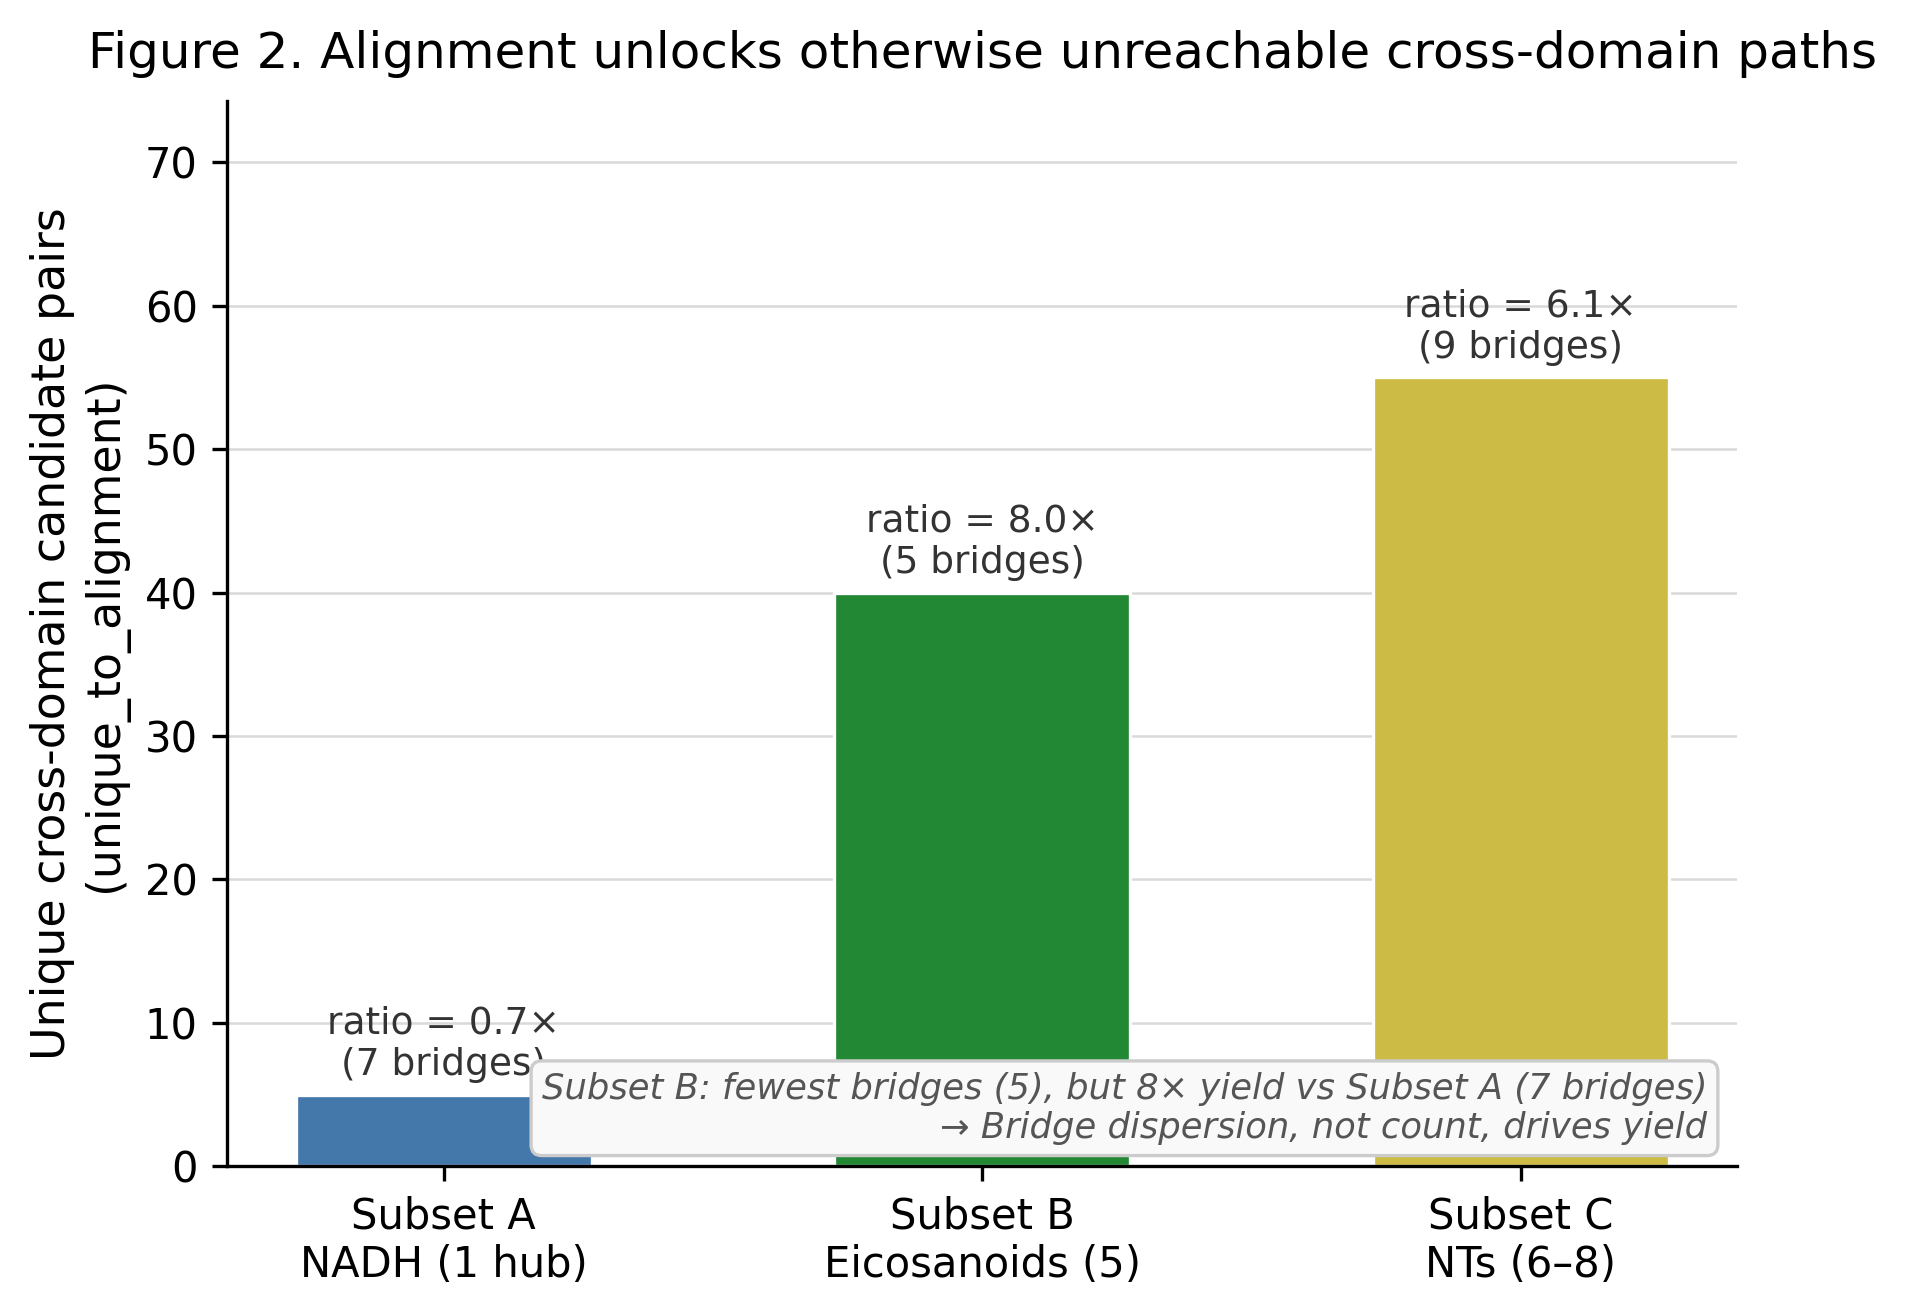
\includegraphics[width=0.88\linewidth]{figures/figure2_alignment_leverage.png}
  \caption{%
    \textbf{Alignment leverage across three domain pairs (Claim 1).}
    Each pair of bars shows total candidates and unique-to-alignment candidates
    for each subset.
    Without alignment (P1 baseline), unique-to-alignment candidates are always zero.
    Bridge count does not predict unique candidate yield: Subset~B (5 bridges) yields
    40 unique pairs while Subset~A (7 bridges) yields only 5, owing to differences in
    bridge structural diversity (Claim 3).
    Error bars not applicable (deterministic runs).
  }
  \label{fig:alignment_leverage}
\end{figure}

Without bridge alignment (P1), the compose operator produces zero cross-domain
candidate pairs across all tested configurations and scales.
With alignment (P4), the pipeline yields between 5 and 55 unique-to-alignment
cross-domain candidates depending on domain pair (Figure~\ref{fig:alignment_leverage}).

Scale amplification is non-linear: a 9$\times$ node increase (57$\to$536 nodes)
with 1.75$\times$ more bridges produces 42$\times$ more unique pairs (4$\to$168).
This is consistent with the theoretical expectation that BFS reachability
through bridge nodes grows with the product of bridge fan-out in both domains.

Run~013 confirms H1'' across all three independent domain pairs
(Table~\ref{tab:subset_comparison}): unique-to-alignment counts are
5 (Subset~A), 40 (Subset~B), and 55 (Subset~C).
The success criterion ($> 0$) is met in 3/3 subsets (confidence: very high).

% Table 2: Subset Comparison
% Source: paper_assets/subset_summary_table.csv
\begin{table}[h]
\caption{%
  \textbf{Subset comparison across three independent domain pairs (Run~013).}
  All three subsets achieve 0\% drift-heavy and 100\% promising rate after
  applying the filter derived from Subset~A without parameter retuning.
  Bridge class diversity, not bridge count, predicts unique candidate yield
  (unique/bridge ratios: 0.7, 8.0, 6.1 for A, B, C respectively).
  Drift-by-depth columns show fraction of candidates at each depth containing
  at least one blocked relation.
}
\label{tab:subset_comparison}
\small
\begin{tabular}{llrrrrrrrrr}
\toprule
 & & \multicolumn{3}{c}{Scale} & \multicolumn{2}{c}{Alignment} & \multicolumn{2}{c}{Filter effect} & \multicolumn{2}{c}{Drift by depth} \\
\cmidrule(lr){3-5}\cmidrule(lr){6-7}\cmidrule(lr){8-9}\cmidrule(lr){10-11}
Sub & Domain pair &
  $|V_{\text{bio}}|$ & $|V_{\text{chem}}|$ & $|V|$ &
  Bridges & Uniq/brdg &
  Raw deep & Filt.\ deep &
  2-hop & 4--5-hop \\
\midrule
A & Cancer sig.\ / Metab.\ chem. &
  293 & 243 & 536 &
  7 & 0.7 &
  20 & 3 &
  8.8\% & 23.7\% \\
B & Immunology / Nat.\ products &
  178 & 110 & 288 &
  5 & 8.0 &
  45 & 39 &
  12.8\% & 29.3\% \\
C & Neurosci.\ / Neuro-pharma. &
  151 & 86  & 237 &
  9 & 6.1 &
  86 & 33 &
  5.6\% & 29.5\% \\
\bottomrule
\end{tabular}

\smallskip
\noindent Uniq/brdg = unique\_to\_alignment candidates per aligned bridge pair.
Raw deep = deep ($\geq$3-hop) cross-domain candidates before filter.
Filt.\ deep = after filter.
Drift-by-depth values for 3-hop not shown; full data in \texttt{paper\_assets/subset\_summary\_table.csv}.
\end{table}


\subsection{Claim 2: Deep Cross-Domain Discovery Is Possible but Requires Quality Filtering}
\label{sec:result-c2}

\begin{figure}[t]
  \centering
  \includegraphics[width=0.88\linewidth]{figures/figure3_drift_by_depth.png}
  \caption{%
    \textbf{Semantic drift rate by path depth across three domain pairs (Claim 2).}
    Drift rate (fraction of candidates containing at least one blocked structural
    relation) increases monotonically with path depth in all three subsets,
    confirming depth-drift as a general structural property of KG composition
    rather than a Subset~A artefact.
    2-hop candidates show the lowest drift ($\leq$12.8\%);
    4--5-hop candidates reach 23--30\% in all subsets.
  }
  \label{fig:drift_by_depth}
\end{figure}

\begin{figure}[t]
  \centering
  \includegraphics[width=0.88\linewidth]{figures/figure4_filter_effect.png}
  \caption{%
    \textbf{Filter effect: before vs.\ after drift filter application (Claim 2).}
    Left: Run~009/011 raw output (Subset~A): 20 deep cross-domain candidates,
    25\% drift-heavy, 15\% promising.
    Right: Run~012 filtered output: 3 candidates, 0\% drift-heavy, 100\% promising.
    No promising candidate is lost by filtering.
    The filter was derived from Subset~A labels and applied unchanged to Subsets~B
    and~C, achieving identical qualitative outcomes (0\% drift / 100\% promising rate).
  }
  \label{fig:filter_effect}
\end{figure}

Without filtering, qualitative review of Run~011's 20 deep cross-domain candidates
(Subset~A) found 25\% drift-heavy and 15\% promising.
Drift-heavy candidates are paths driven by structural chemical relations
(e.g., \texttt{contains}, \texttt{is\_product\_of}) that express molecular facts
rather than mechanistic hypotheses.

The Run~012 drift filter reduces deep candidates from 20 to 3,
achieving 0\% drift-heavy and 100\% promising.
Critically, \textbf{no promising candidate is lost}: all three
VHL/HIF1A/LDHA cascade candidates pass the filter
(Figure~\ref{fig:filter_effect}).

Figure~\ref{fig:drift_by_depth} shows that drift rate increases monotonically with
path depth across all three subsets.
At 2-hop depth: 8.8--12.8\% drift rate.
At 4--5-hop depth: 23.7--29.5\%.
This monotonic relationship holds without exception across the three domain pairs,
confirming that depth-drift is a general structural property of KG composition.

\paragraph{Filter generalisation.}
Subsets~B and~C, with entirely different chemistry, achieve identical qualitative
outcomes (0\% drift-heavy, 100\% promising rate) when the Subset~A-derived filter
is applied without parameter adjustment.
Subset~B yields 39 filter-passing deep cross-domain candidates;
Subset~C yields 33.

\paragraph{H4 auxiliary: provenance-aware ranking.}
The revised traceability scorer (Run~010) promotes 309 deep candidates
vs.\ 209 demoted (net +100; Jaccard similarity to naive ranking: 0.429).
However, top-20 composition remains 2-hop only in all subsets and all
scoring configurations (mean score across subsets: 0.78).
Deep candidates require supplementary depth-promotion or a minimum-depth
tier in the ranking to surface in practical use.
This is an open problem (Section~\ref{sec:limitations}).

\subsection{Claim 3: Bridge Dispersion, Not Bridge Count, Drives Candidate Yield}
\label{sec:result-c3}

The unique-to-alignment ratios per bridge pair are 0.7 (Subset~A), 8.0 (Subset~B),
and 6.1 (Subset~C).
This ordering does not follow bridge count (7 bridges $\to$ 0.7$\times$;
5 bridges $\to$ 8.0$\times$; 9 bridges $\to$ 6.1$\times$).

The consistent predictor is bridge entity structural diversity:
\begin{itemize}[noitemsep]
  \item Subset~A: NADH (single metabolic hub with limited fan-out in both domains)
    $\to$ 5 unique pairs from 7 bridges
  \item Subset~B: five eicosanoids (AA, PGE$_2$, LTB$_4$, PGI$_2$, TXA$_2$;
    each connects to multiple downstream synthesis enzymes and natural product targets)
    $\to$ 40 unique pairs from 5 bridges
  \item Subset~C: 6--8 neurotransmitters (Dopamine, Serotonin, GABA, NE, \ldots;
    each connects to synthesis genes \textit{and} drug targets in both domains)
    $\to$ 55 unique pairs from 9 bridges
\end{itemize}

This finding is observational and based on three data points (see Threat~T3.1);
it establishes a directional hypothesis---bridge dispersion predicts yield
better than bridge count---that warrants formal quantification in future work.
